% SPDX-License-Identifier: Apache-2.0 OR MIND-UCAL-1.0
% © James Ross Ω FLYING•ROBOTS <https://github.com/flyingrobots>
% BOAW Pipeline Diagram - Standalone TikZ
\documentclass[tikz,border=8pt]{standalone}
\usepackage[T1]{fontenc}
\usepackage{lmodern}
\usetikzlibrary{arrows.meta,positioning,fit,calc}
\begin{document}
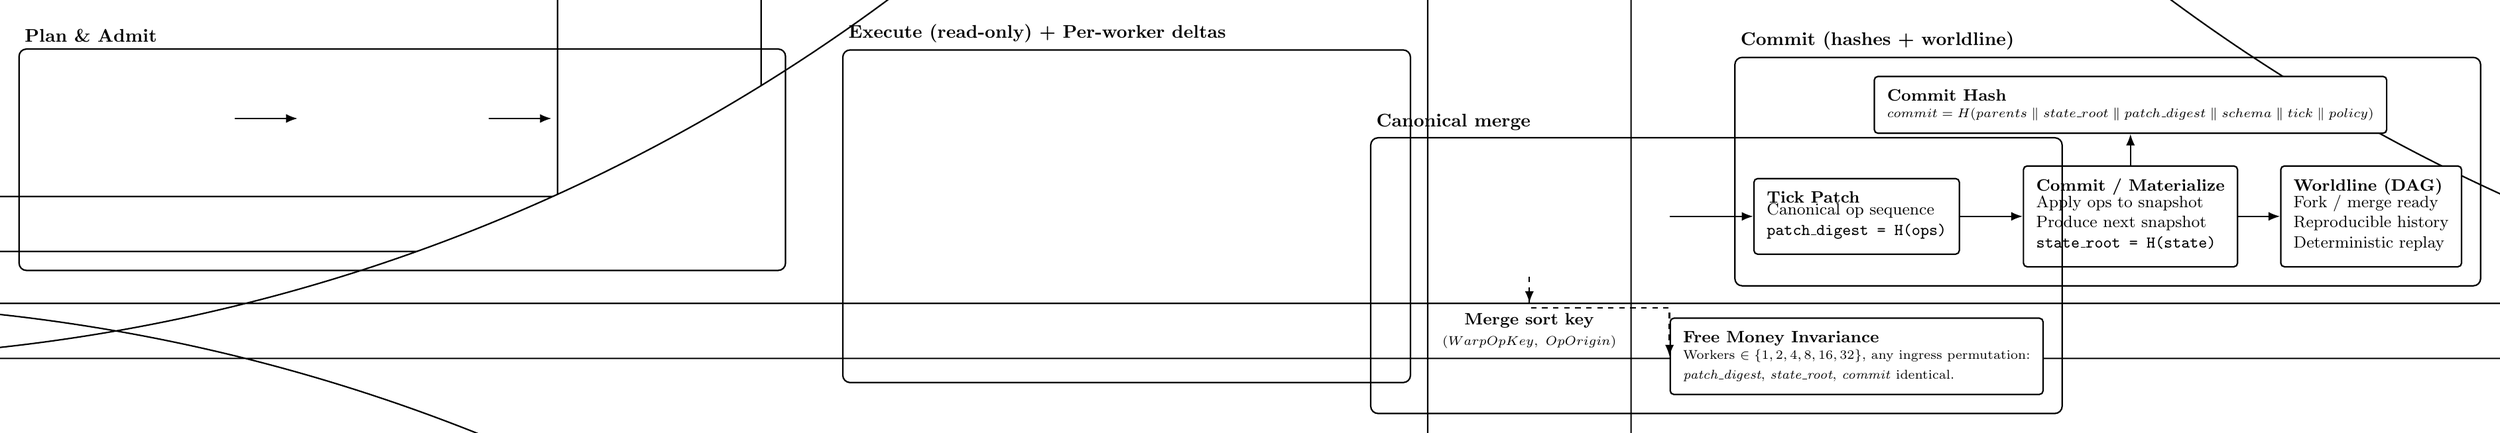
\begin{tikzpicture}[
  font=\small,
  >=Latex,
  node distance=10mm and 12mm,
  block/.style={draw, rounded corners=2pt, thick, align=left, inner xsep=7pt, inner ysep=7pt, fill=white},
  pill/.style={draw, rounded corners=999pt, thick, inner xsep=8pt, inner ysep=4pt, fill=white},
  group/.style={draw, rounded corners=4pt, thick, inner xsep=10pt, inner ysep=10pt},
  arrow/.style={thick, -{Latex[length=2.2mm,width=1.7mm]}},
  dashedarrow/.style={thick, dashed, -{Latex[length=2.2mm,width=1.7mm]}}
]
% Plan and Admit
\node[block] (ingress) {\textbf{Ingress (canonical)}\\[-2pt]\begin{tabular}{@{}l@{}}Intents $\rightarrow$ \emph{intent\_id}\\Stable ordering (radix)\end{tabular}};
\node[block, right=of ingress] (plan) {\textbf{Plan}\\[-2pt]\begin{tabular}{@{}l@{}}Match on \texttt{GraphView}\\Compute \emph{Footprint}\\Emit \texttt{PlannedRewrite}\end{tabular}};
\node[block, right=of plan] (admit) {\textbf{Admit (deterministic)}\\[-2pt]\begin{tabular}{@{}l@{}}Greedy, canonical order\\Footprint independence\\Output: \texttt{ExecItem} list\end{tabular}};
\node[pill, below=5mm of admit] (admitkey) {\begin{tabular}{@{}c@{}}\textbf{Admission order}\\\scriptsize $(scope\_hash,\ rule,\ nonce)$\end{tabular}};
\draw[arrow] (ingress) -- (plan);
\draw[arrow] (plan) -- (admit);
\draw[dashedarrow] (admit) -- (admitkey);
% Execute
\node[block, right=18mm of admit] (snapshot) {\textbf{Base Snapshot}\\[-2pt]\begin{tabular}{@{}l@{}}Reachable-only view\\WSC / zero-copy IO\\\texttt{GraphView} reads only\end{tabular}};
\node[block, below=6mm of snapshot] (execitems) {\textbf{ExecItem list}\\[-2pt]\begin{tabular}{@{}l@{}}\texttt{exec: ExecuteFn}\\\texttt{scope: NodeId}\\\texttt{origin: OpOrigin}\end{tabular}};
\draw[arrow] (admit) -- (snapshot);
\draw[arrow] (admit) -- (execitems);
\node[block, right=16mm of snapshot] (w0) {\textbf{Worker 0}\\[-2pt]\begin{tabular}{@{}l@{}}Read: \texttt{GraphView}\\Write: \texttt{TickDelta\_0}\end{tabular}};
\node[block, below=4mm of w0] (w1) {\textbf{Worker 1}\\[-2pt]\begin{tabular}{@{}l@{}}Read: \texttt{GraphView}\\Write: \texttt{TickDelta\_1}\end{tabular}};
\node[block, below=4mm of w1] (wk) {\textbf{Worker $\dots$}\\[-2pt]\begin{tabular}{@{}l@{}}Read: \texttt{GraphView}\\Write: \texttt{TickDelta\_k}\end{tabular}};
\draw[arrow] (snapshot.east) -- ++(7mm,0) |- (w0.west);
\draw[arrow] (snapshot.east) -- ++(7mm,0) |- (w1.west);
\draw[arrow] (snapshot.east) -- ++(7mm,0) |- (wk.west);
\draw[arrow] (execitems.east) -- ++(7mm,0) |- (w0.west);
\draw[arrow] (execitems.east) -- ++(7mm,0) |- (w1.west);
\draw[arrow] (execitems.east) -- ++(7mm,0) |- (wk.west);
\node[block, below=6mm of w1] (origin) {\textbf{Origin tie-break}\\[-2pt]\scriptsize \texttt{OpOrigin = (intent\_id, rule\_id, match\_ix, op\_ix)}\\\scriptsize \texttt{op\_ix} assigned by scoped emission};
% Merge
\node[block, right=16mm of w1] (merge) {\textbf{Canonical Merge}\\[-2pt]\begin{tabular}{@{}l@{}}Flatten all \texttt{TickDelta}s\\Sort by $(WarpOpKey, OpOrigin)$\\Dedupe identical ops\\Explode on divergence\end{tabular}};
\draw[arrow] (w0.east) -- (merge.west);
\draw[arrow] (w1.east) -- (merge.west);
\draw[arrow] (wk.east) -- (merge.west);
\node[pill, below=5mm of merge] (mergekey) {\begin{tabular}{@{}c@{}}\textbf{Merge sort key}\\\scriptsize $(WarpOpKey,\ OpOrigin)$\end{tabular}};
\draw[dashedarrow] (merge) -- (mergekey);
% Commit
\node[block, right=16mm of merge] (patch) {\textbf{Tick Patch}\\[-2pt]\begin{tabular}{@{}l@{}}Canonical op sequence\\\texttt{patch\_digest = H(ops)}\end{tabular}};
\node[block, right=of patch] (build) {\textbf{Commit / Materialize}\\[-2pt]\begin{tabular}{@{}l@{}}Apply ops to snapshot\\Produce next snapshot\\\texttt{state\_root = H(state)}\end{tabular}};
\node[block, above=6mm of build] (chash) {\textbf{Commit Hash}\\[-2pt]\scriptsize $commit = H(parents \parallel state\_root \parallel patch\_digest \parallel schema \parallel tick \parallel policy)$};
\node[block, right=8mm of build] (dag) {\textbf{Worldline (DAG)}\\[-2pt]\begin{tabular}{@{}l@{}}Fork / merge ready\\Reproducible history\\Deterministic replay\end{tabular}};
\draw[arrow] (merge) -- (patch);
\draw[arrow] (patch) -- (build);
\draw[arrow] (build) -- (chash);
\draw[arrow] (build) -- (dag);
% Invariance
\node[block, below=12mm of patch, align=left] (invar) {\textbf{Free Money Invariance}\\[-2pt]\scriptsize Workers $\in \{1,2,4,8,16,32\}$, any ingress permutation:\\\scriptsize \emph{patch\_digest}, \emph{state\_root}, \emph{commit} identical.};
\draw[dashedarrow] (merge.south) -- ++(0,-6mm) -| (invar.west);
% Group frames
\node[group, fit=(ingress)(plan)(admit)(admitkey)] (g1) {};
\node[group, fit=(snapshot)(execitems)(w0)(w1)(wk)(origin)] (g2) {};
\node[group, fit=(merge)(mergekey)(invar)] (g3) {};
\node[group, fit=(patch)(build)(chash)(dag)] (g4) {};
\node[font=\bfseries, anchor=south west] at (g1.north west) {Plan \& Admit};
\node[font=\bfseries, anchor=south west] at (g2.north west) {Execute (read-only) + Per-worker deltas};
\node[font=\bfseries, anchor=south west] at (g3.north west) {Canonical merge};
\node[font=\bfseries, anchor=south west] at (g4.north west) {Commit (hashes + worldline)};
\end{tikzpicture}
\end{document}
